\documentclass[border=15pt]{standalone}
\usepackage{tikz,amsmath}
\usetikzlibrary{arrows.meta}

\definecolor{inFill}{RGB}{183,224,177}
\definecolor{inLine}{RGB}{32,102,32}
\definecolor{outLine}{RGB}{143,52,52}

\begin{document}
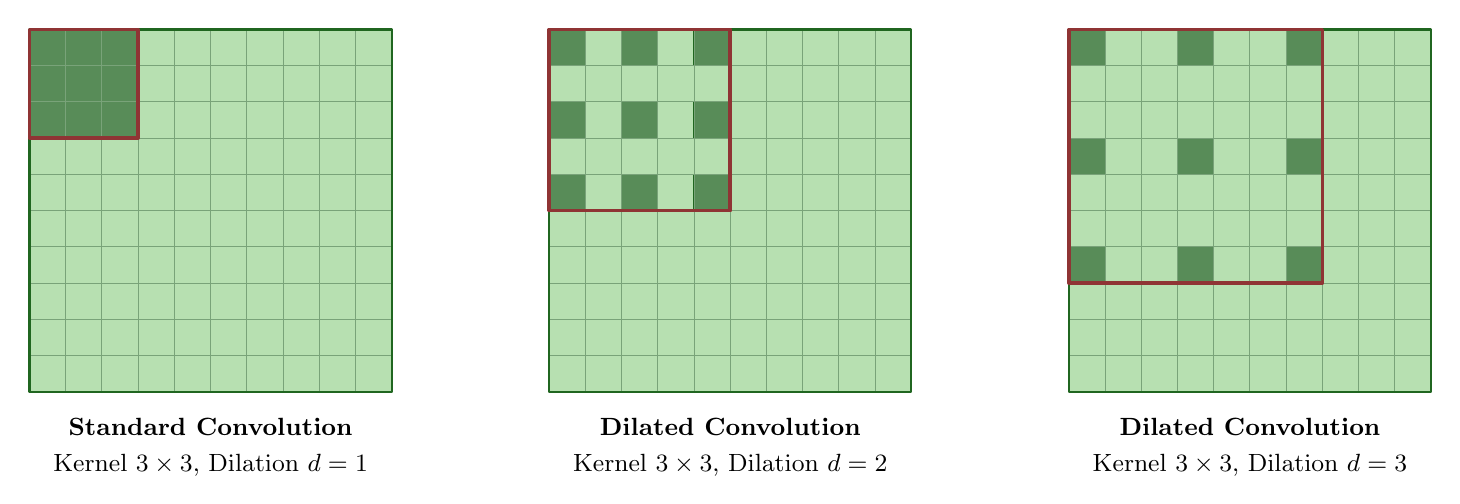
\begin{tikzpicture}[
    font=\small, line join=round,
    every node/.style={inner sep=0pt, outer sep=0pt, align=center}
  ]

  % 左侧：标准卷积输入 (10x10，感受野 3x3，d=1)
  \fill[inFill] (0, -2.3) rectangle ++(4.6, 4.6);

  % 左侧连续 3x3 采样格深色填充
  \foreach \r in {0,1,2} {
    \foreach \c in {0,1,2} {
      \fill[inLine!75] ({0 + \c*0.46}, {2.3 - (\r+1)*0.46}) rectangle ++(0.46, 0.46);
      \draw[inLine, line width=.4pt] ({0 + \c*0.46}, {2.3 - (\r+1)*0.46}) rectangle ++(0.46, 0.46);
    }
  }

  % 左侧网格线与外边框
  \draw[step=0.46, inLine!60, line width=.35pt] (0, -2.3) grid ++(4.6, 4.6);
  \draw[inLine, thick] (0, -2.3) rectangle ++(4.6, 4.6);

  % 左侧 3x3 感受野红框
  \draw[outLine, line width=1.3pt] (0, 0.92) rectangle (1.38, 2.3);

  % 左侧底部标题与说明
  \node[align=center] at (2.3, -3.0) {
    \textbf{Standard Convolution}\\[2pt]
    Kernel $3\times 3$, Dilation $d=1$
  };

  % 中间：空洞卷积输入 (10x10，感受野 5x5，d=2)
  \fill[inFill] (6.6, -2.3) rectangle ++(4.6, 4.6);

  % 中间 9 个带孔采样格深色填充 (步长为 2)
  \foreach \r in {0,2,4} {
    \foreach \c in {0,2,4} {
      \fill[inLine!75] ({6.6 + \c*0.46}, {2.3 - (\r+1)*0.46}) rectangle ++(0.46, 0.46);
      \draw[inLine, line width=.4pt] ({6.6 + \c*0.46}, {2.3 - (\r+1)*0.46}) rectangle ++(0.46, 0.46);
    }
  }

  % 中间网格线与外边框
  \draw[step=0.46, inLine!60, line width=.35pt, shift={(6.6, -2.3)}] (0, 0) grid ++(4.6, 4.6);
  \draw[inLine, thick] (6.6, -2.3) rectangle ++(4.6, 4.6);

  % 中间 5x5 跨度感受野红框
  \draw[outLine, line width=1.3pt] (6.6, 0) rectangle (8.9, 2.3);

  % 中间底部标题与说明
  \node[align=center] at (8.9, -3.0) {
    \textbf{Dilated Convolution}\\[2pt]
    Kernel $3\times 3$, Dilation $d=2$
  };

  % 右侧：空洞卷积输入 (10x10，感受野 7x7，d=3)
  \fill[inFill] (13.2, -2.3) rectangle ++(4.6, 4.6);

  % 右侧 9 个带孔采样格深色填充 (步长为 3)
  \foreach \r in {0,3,6} {
    \foreach \c in {0,3,6} {
      \fill[inLine!75] ({13.2 + \c*0.46}, {2.3 - (\r+1)*0.46}) rectangle ++(0.46, 0.46);
      \draw[inLine, line width=.4pt] ({13.2 + \c*0.46}, {2.3 - (\r+1)*0.46}) rectangle ++(0.46, 0.46);
    }
  }

  % 右侧网格线与外边框
  \draw[step=0.46, inLine!60, line width=.35pt, shift={(13.2, -2.3)}] (0, 0) grid ++(4.6, 4.6);
  \draw[inLine, thick] (13.2, -2.3) rectangle ++(4.6, 4.6);

  % 右侧 7x7 跨度感受野红框 (7格跨度 = 3.22cm)
  \draw[outLine, line width=1.3pt] (13.2, -0.92) rectangle (16.42, 2.3);

  % 右侧底部标题与说明
  \node[align=center] at (15.5, -3.0) {
    \textbf{Dilated Convolution}\\[2pt]
    Kernel $3\times 3$, Dilation $d=3$
  };

\end{tikzpicture}
\end{document}